\section{Mockups}

\begin{figure}[H]
	\centering
	\begin{subfigure}{.4\textwidth}
		\centering
		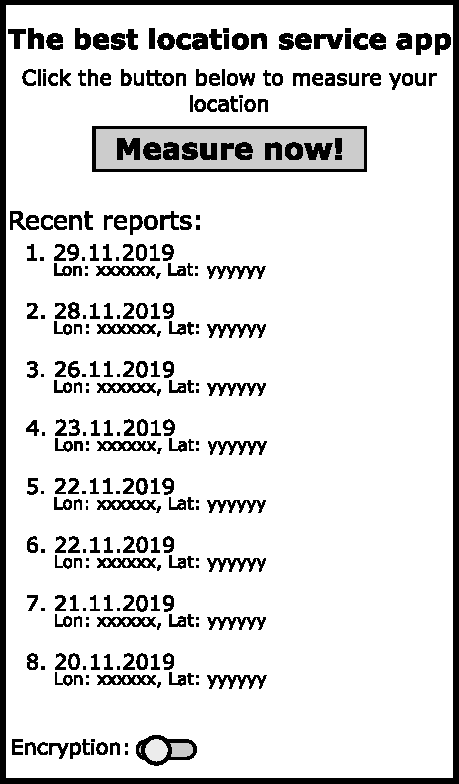
\includegraphics[width=.8\textwidth]{graphics/mockupmainfragment}
		\caption{Mockup Hauptbildschirm}
		\label{fig:mockHaupt}
	\end{subfigure}
	\begin{subfigure}{.4\textwidth}
		\centering
		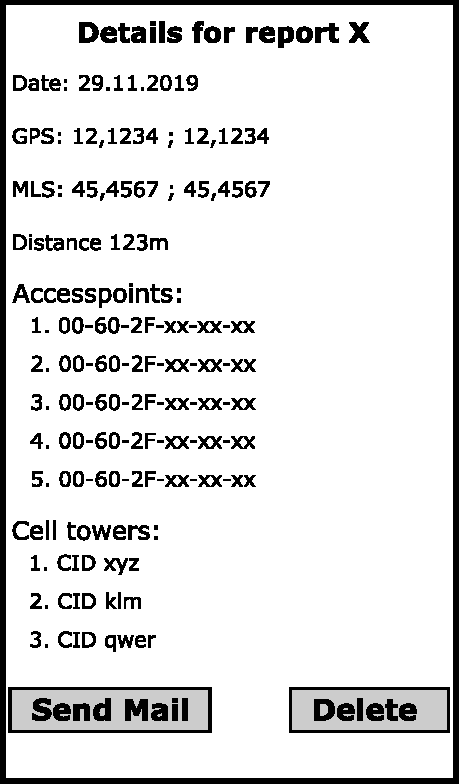
\includegraphics[width=.8\textwidth]{graphics/mockupdetailfragment}
		\caption{Mockup Detailansicht}
		\label{fig:mockDetail}
	\end{subfigure}
	\caption{Porträt Mockups der Compare Location App}
\end{figure}

\begin{figure}
	\centering
	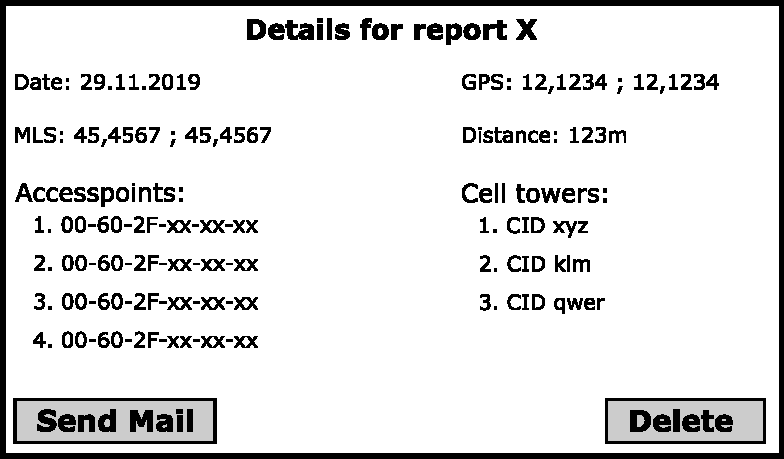
\includegraphics[width=.6\textwidth]{graphics/mockupdetailfragmentlandscape}
	\caption{Mockup Detailansicht Landscape Modus}
	\label{fig:mockDetailLand}
\end{figure}


Mockups wurden mit Inkscape erstellt. Abbildung \ref{fig:mockHaupt} zeigt die Hauptansicht der App mit einer Schaltfläche zum Starten einer Messung, einer Liste mit den Messberichten und einem Schalter zur Aktivierung der Verschlüsselung der Datenbank. In der Detailansicht \ref{fig:mockDetail} werden unter anderem die ermittelten Koordinaten, eine Liste der verwendeten WLAN Stationen sowie eine Liste der Mobilfunksender angezeigt. Des Weiteren, finden sich hier zwei Schaltflächen, die es erlauben den Bericht zu löschen oder ihn als E-Mail zu verschicken. Der Panoramamodus der Detailansicht ist in \ref{fig:mockDetailLand} zu sehen. Die Elemente sind dieselben wie im Porträtmodus, nur die Anordnung ändert sich.